\documentclass{article}
\usepackage[margin=1in]{geometry}
\usepackage{mathtools, amsfonts, amsthm, graphicx, listings, xcolor, tikz}

% \setlength\parindent{0pt}

\definecolor{codegreen}{rgb}{0,0.6,0}
\definecolor{codegray}{rgb}{0.5,0.5,0.5}
\definecolor{codepurple}{rgb}{0.58,0,0.82}
\definecolor{backcolour}{rgb}{0.95,0.95,0.92}

\lstdefinestyle{mystyle}{
    backgroundcolor=\color{backcolour},   
    commentstyle=\color{codegreen},
    keywordstyle=\color{magenta},
    numberstyle=\tiny\color{codegray},
    stringstyle=\color{codepurple},
    basicstyle=\ttfamily\footnotesize,
    breakatwhitespace=false,         
    breaklines=true,                 
    captionpos=b,                    
    keepspaces=true,                 
    numbers=left,                    
    numbersep=5pt,                  
    showspaces=false,                
    showstringspaces=false,
    showtabs=false,                  
    tabsize=2
}

\lstset{style=mystyle}

\title{HW04}
\author{Sam Ly}

\begin{document}
\maketitle

\section*{Total Points: 21}

\section*{Required Exercise 1 [2]}

\begin{enumerate}
    \item Did it.
    \item Did it.
\end{enumerate}


\section*{Required Exercise 2 [1]}

\begin{itemize}
    \item {
        In class during week 4, we proved that since my birthday was on a Saturday this year (2025), it will be on a Sunday next year (2026). We did this by showing that
        \[x + 365 \equiv x + 1 \pmod{7}\]
        Why does this prove the claim?

        This proves the claim because all ``days of the week'' are actually 
        individual congruency classes \(\pmod{7}\). Thus, when we add the no. of 
        days equal to a year (365), and find that it is congruent to 1 \(\pmod{7}\),
        we are saying that moving a year forward puts use in the same congruency 
        class of days of the week as moving one day forward. Thus, if your birthday
        was on a Saturday this year, it will be on a Sunday next year.
    }

    \item {
        We also showed that if the minute hand of the clock says now, then in 
        minutes, it will say by showing that
        \[19 + 52 \equiv 11 \pmod{60}\]

        This proves the claim because of similar reasoning as the prior exercise. 
        Each second of the minute can be seen as a congruency class, and by seeing 
        that \(19 + 52 \equiv 11 \pmod{60}\), we see that the second hand will be 
        on the 11 seconds mark.
    }
\end{itemize}

\section*{Required Exercise 3 [3]}

\begin{enumerate}
    \item {
        Prove that if all the coefficients of the quadratic equation
        \[ax^2 + bx + c = 0\]
        are odd integers, then the roots of the equation cannot be rational.

        \begin{proof}
            We begin by seeing that the roots of a quadratic equation are
            \[\frac{-b \pm \sqrt{b^2 - 4ac}}{2a}.\]

            This expression is not rational if \(b^2 - 4ac\) is not square. We also see 
            that \(b^2 - 4ac\) must be odd because \(b^2\) is odd, and \(4ac\) is even, 
            and an odd number minus an even number is always odd. 

            \begin{description}
                \item[Lemma 1] {
                    Let \(m\) be an odd integer. \(m^2 \equiv 1 \pmod{8}\).
                
                    Since \(m\) is odd, it must have the form \(2k + 1\) for some 
                    integer \(k\). Thus, all odd squares can b written in the as
                    \[(2k+1)^2 = 4k^2 + 4k + 1 = 4(k^2 + k) + 1.\]

                    Now, we see that \(k^2 + k\) must always be even, because if 
                    \(k\) was odd, \(k^2\) would also be odd, and an odd plus odd
                    is always even, and if \(k\) was even, then \(k^2\) is even,
                    and an even plus even is always even. Thus, \(k^2 + k\) can 
                    be written in the form \(2j\) for some integer \(j\).

                    By substituting, we get 
                    \[4(k^2 + k) + 1 = 4(2j) + 1 = 8j + 1.\]
                    And \(8j + 1 \equiv 1 \pmod{8}\) because \(8 \mid (8j + 1 - 1) \).

                    Thus, for any odd square \(n\), \(n \equiv 1 \pmod{8}\). \qed
                }
            \end{description}

            Now, using the contrapositive of \textbf{Lemma 1}, we see that for 
            any integer \(k \not\equiv 1 \pmod{8}\), \(k\) must not be an odd square.

            Let \(a = 2k_1 + 1\), \(b = 2k_2 + 1\), and \(c = 2k_3 + 1\).
            By substituting into \(b^2 - 4ac\) and algebraic manipulation, we get 
            \[4{k_2}^2 + 4k_2 + 1 - 4(4k_1k_3 + 2k_1 + 2k_3 + 1)\]
            \[4{k_2}^2 + 4k_2 + 1 - 16k_1k_3 -8k_1 - 8k_3 - 4\]
            \[4{k_2}^2 + 4k_2 - 16k_1k_3 -8k_1 - 8k_3 - 3\]
            \[4 ({k_2}^2 + k_2 - 4k_1k_3 - 2k_1 - 2k_3) - 3.\]
            
            Then, notice that \({k_2}^2 + k_2\) is always even because if 
            \(k_2\) was odd, \({k_2}^2\) would also be odd, and an odd plus odd
            is always even, and if \(k_2\) was even, then \({k_2}^2\) is even,
            and an even plus even is always even.

            Also, notice that \(4k_1k_3 -2k_1 -2k_3\) is always even because
            a it can be written in the form 
            \[2(2k_1k_3 - k_1 -k_3).\]

            Now, we can see that the entire expression \({k_2}^2 + k_2 - 4k_1k_3 - 2k_1 - 2k_3\)
            must be even. 
            
            Thus, \({k_2}^2 + k_2 - 4k_1k_3 - 2k_1 - 2k_3 = 2i\) 
            for some integer \(i\).

            Finally, can substitute our new expression to see
            \[4 ({k_2}^2 + k_2 - 4k_1k_3 - 2k_1 - 2k_3) - 3 = 4 (2i) - 3 = 8i - 3.\]

            For any integer \(i\), \(8i -3 \not\equiv 1 \pmod{8}\). 
            Since \(b^2 - 4ac \not\equiv 1 \pmod{8}\) and \(b^2 -4ac\) is odd, 
            \(b^2 - 4ac\) can not be square. Thus, the roots of the quadratic
            equation \(ax^2 + bx + c\) cannot be rational.

        \end{proof}

    }
\end{enumerate}

\section*{Required Exercise 4 [4]}

\begin{enumerate}
    \item {
        Solve the following three questions about set complements.

        \begin{itemize}
            \item {
                Suppose that \(\mathcal{O}\) is the set of odd integers. If 
                \(\mathcal{U} = \mathbb{Z}\) (the set of integers), what is
                \(\mathcal{O}^c\)?

                All integers can be classified as either even or odd. All integers 
                that are even are not odd, and all the integers that are odd are not
                even. Thus, \(\mathcal{O}^c\) is the set of all integers that are 
                not odd, which is just the set of all even integers 
                \(\mathcal{E} = \{2n : n \in \mathbb{Z}\}\).
            }

            \item {
                Suppose that \(A = \{1, 2, 3, 5, 8\}\) and the universal set is 
                \(\mathcal{U} = {1,2,...,10}\). What is \(A^c\)?

                \(A^c\) is the set of numbers in \(\mathcal{U}\) that are not in 
                \(A\). Thus, \(A^c = {4, 6, 7, 9}\).
            }

            \item {
                Suppose that \(B = \{(x,y) \in \mathbb{R} \times \mathbb{R} : x^2 + y^2 > 1\}\)
                and \(\mathcal{U} = \mathbb{R} \times \mathbb{R}\). What is \(B^c\)?

                The set \(B\) is the set of all points that lie strictly outside 
                the unit circle on the Cartesian plane, thus the complement of 
                this set \(B^c \) is the set of all points inside or on the unit 
                circle. In other words, \(B^c = \{(x,y) \in \mathbb{R}^2 : x^2 + y^2 \le 1\}\).
            }
        \end{itemize}
    }

    \item {
        Now prove De Morgan's laws. In both cases, assume that \(A\) and \(B\) are 
        both subsets of the universal set \(\mathcal{U}\).

        \emph{I will be using \(\subset\) to be "proper subset".}

        \begin{itemize}
            \item {
                \((A \cup B)^c = A^c \cap B^c\)
                \begin{proof}
                    We begin by seeing that for any two sets \(X\) an \(Y\), if \(X \subseteq Y\) 
                    and \(Y \subseteq X\), then \(X = Y\).

                    Suppose \(x \in (A \cup B)^c\), so \(x \not\in A\), and thus \(x \in A^c\). 
                    Similarly,  \(x \not\in B\), and thus \(x \in B^c\).

                    Therefore, for every \(x \in (A \cup B)^c\), \(x \in A^c \cap B^c\).
                    So, \((A \cup B)^c \subseteq A^c \cap B^c\).

                    Now, suppose \(x \in A^c \cap B^c\), so \(x \not\in A\), and thus \(x \in A^c\). 
                    Similarly,  \(x \not\in B\), and thus \(x \in B^c\).

                    Therefore, for every \(x \in A^c \cap B^c\), \(x \in (A \cup B)^c\).
                    So, \( A^c \cap B^c \subseteq (A \cup B)^c \).

                    Because both \( A^c \cap B^c \subseteq (A \cup B)^c \) and 
                    \((A \cup B)^c \subseteq A^c \cap B^c\), \((A \cup B)^c = A^c \cap B^c\).
                \end{proof}
            }

            \item 
                \((A \cap B)^c = A^c \cup B^c\)
                \begin{proof}
                    We begin by seeing that for any two sets \(X\) an \(Y\), if \(X \subseteq Y\) 
                    and \(Y \subseteq X\), then \(X = Y\).

                    Suppose \(x \in (A \cap B)^c\), so \(x\) can't be in both \(A\) 
                    and \(B\) at the same time. Thus, \(x \in A^c \cup B^c\).

                    Therefore, for every \(x \in (A \cap B)^c\), \(x \in A^c \cup B^c\).
                    So, \((A \cap B)^c \subseteq A^c \cup B^c\).

                    Now, suppose \(x \in A^c \cup B^c\), so \(x \in (\mathcal{U} \setminus A) \cup(\mathcal{U} \setminus B) \).
                    If we let \(x\) be an element of \(B\), we see that this must come from the complement of \(A\).
                    Similarly, if we let \(x \in A\), we see that \(x \in B^c\).
                    In other words, \(x\) can't be in \(A\) and \(B\) at the same time. 

                    Therefore, for every \(x \in A^c \cup B^c\), \(x \in (A \cap B)^c\).
                    So, \( A^c \cup B^c \subseteq (A \cap B)^c \).

                    Because both \( A^c \cup B^c \subseteq (A \cap B)^c \) and 
                    \((A \cap B)^c \subseteq A^c \cup B^c\), \((A \cap B)^c = A^c \cup B^c\).
                \end{proof}
        \end{itemize}
    }
\end{enumerate}

\section*{Choice Exercise 9 [4]}

I really enjoyed the premise of this video and I feel like I've got a decent 
intuition for the problem. I understood the ``mapping'' of the original problem to 
the problem of coloring some n-dimensional cube. Because I have a CS background, 
graph theory problems are somewhat familiar to me, so reasoning about the coloring 
point of view wasn't too foreign. However, the combinitorical proof for showing 
only cases where the no. of squares is a power of two are even possible was a little 
bit confusing. I get the concrete example with a 3D cube where we literally can't 
evenly partition the colors, but I struggle to comprehend the generallization to 
higher dimensions. After watching, I wonder what if instead of having coins on 
the chessboard, what if we had n-sided ``dice'' where the position can be any 
value from one to n. Now, with this variant, we can either limit the ways we can 
manipulate the dice (only increase or decrease value by 1), or let us arbitrarily 
set the value. 

Just writing this description, I can already sort of see that for n-sided dice 
where n is a power of 2 is essentially the same as our original problem in special 
cases, because the n-sided dice is equal to \(log(n)\) squares worth of information. 
There seems to be more to this problem, but I'm struggling to articulate everything 
because I feel as though I don't have the language to convey the ideas. 

Even stranger still if we can extend the values to the Reals. I don't know if 
this problem even makes sense to ask. 

\section*{Choice Exercise 10 [3]}

\begin{description}
    \item[My drawing] {
        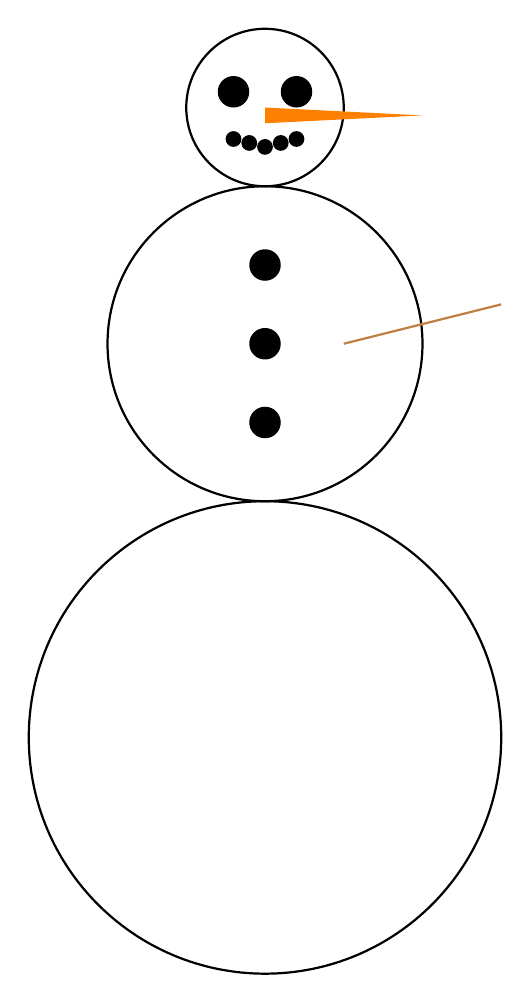
\begin{tikzpicture}

        \draw[thick, black] (1,0) circle (1);
        \fill[black] (0.6, 0.2) circle (0.2);
        \fill[black] (1.4, 0.2) circle (0.2);
        \fill[orange] (1, 0)--(1, -0.2)--(3,-0.1);
        \fill[black] (1, -0.5) circle (0.1);
        \fill[black] (1.2, -0.45) circle (0.1);
        \fill[black] (0.8, -0.45) circle (0.1);
        \fill[black] (1.4, -0.4) circle (0.1);
        \fill[black] (0.6, -0.4) circle (0.1);

        \draw[thick, black] (1,-3) circle (2);
        \fill[black] (1, -2) circle (0.2);
        \fill[black] (1, -3) circle (0.2);
        \fill[black] (1, -4) circle (0.2);

        \draw[thick, brown] (2, -3) -- (4, -2.5);

        \draw[thick, black] (1,-8) circle (3);
        \end{tikzpicture}

        Not too shabby for an 8 minute drawing if I do say so myself.
    }

    \item[ChatGPT's drawing] {
        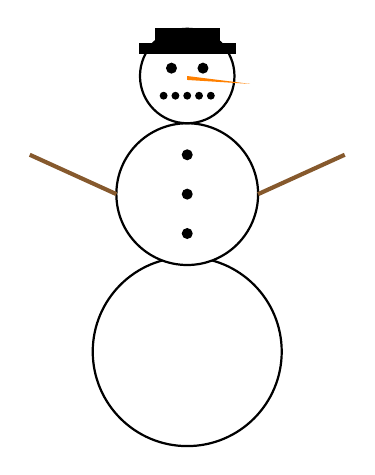
\begin{tikzpicture}[thick]

        % Body
        \draw[fill=white] (0,0) circle (1.2);
        \draw[fill=white] (0,2) circle (0.9);
        \draw[fill=white] (0,3.5) circle (0.6);

        % Eyes
        \fill (-0.2,3.6) circle (0.07);
        \fill (0.2,3.6) circle (0.07);

        % Nose
        \fill[orange] (0,3.5) -- (0.8,3.4) -- (0,3.45) -- cycle;

        % Mouth
        \foreach \x in {-0.3,-0.15,0,0.15,0.3}
        \fill (\x,3.25) circle (0.05);

        % Buttons
        \foreach \y in {2.5,2.0,1.5}
        \fill (0,\y) circle (0.07);

        % Arms
        \draw[brown!70!black,line width=1.5pt] (0.9,2) -- (2,2.5);
        \draw[brown!70!black,line width=1.5pt] (-0.9,2) -- (-2,2.5);

        % Hat
        \draw[fill=black] (-0.4,4.1) rectangle (0.4,3.9);
        \draw[fill=black] (-0.6,3.9) rectangle (0.6,3.8);

        \end{tikzpicture}
    }

    \item[Analysis] Damn I got cooked.
\end{description}

\section*{Choice Exercise 11 [4]}

\begin{enumerate}
    \item {
        How do the roots that I got compare with the roots you get when you use 
        the quadratic formula on the polynomial \(2x^2 -5x + 6\)?

        Using the quadratic equation, we get
        \[x = \frac{5 \pm \sqrt{25 - 4(2(6))}}{2(2)} = \frac{5 \pm \sqrt{-23}}{4}.\]

        This is the same as our result from completing the square.
    }

    \item {
        Do the same process again, but where the quadratic polynomial has coefficients 
        \(a\), \(b\), and  \(c\).

        \[ax^2 + bx + c = 0\]
        \[x^2 + \frac{b}{a}x + \frac{c}{a} = 0\]
        \[x^2 + \frac{b}{a}x = -\frac{c}{a}\]
        \[x^2 + \frac{b}{a}x + \left(\frac{b}{2a}\right)^2= -\frac{c}{a} + \left(\frac{b}{2a}\right)^2\]
        \[\left(x + \frac{b}{2a} \right)^2 = -\frac{4ac}{4a^2} + \frac{b^2}{4a^2} = \frac{b^2 - 4ac}{4a^2}\]
        
        \[x + \frac{b}{2a}  =  \frac{\pm \sqrt{b^2 - 4ac}}{2a}\]
        \[x =  \frac{-b \pm \sqrt{b^2 - 4ac}}{2a}.\]

        We have derived the quadratic formula.
    }
\end{enumerate}
\end{document}